\documentclass[%draft,
    11pt, % use explicit paper size
    headinclude, footexclude,
    % twoside, % this produces strange margins!
    openright, % for new chapters
    notitlepage,
    cleardoubleempty,
    headsepline,
    pointlessnumbers,
    bibtotoc, idxtotoc,
    ]{scrbook}

% LeeSeshia is 15,73 ? 20,96 cm
% that was for CreateSpace trim size of JOP book
% \setlength{\paperwidth}{7.5in} \setlength{\paperheight}{9.25in}
% \typearea[0.5in]{14}
% This results in 19,05 ? 23,5 cm
\setlength{\paperwidth}{15cm} \setlength{\paperheight}{20cm}
%\typearea{calc} % without BCOR results to a DIV of 8 for 11pt
\typearea[1cm]{16} % TODO: check if 1 cm is the correct number

% I should switch:
% From KOMA-Script 3.12 the completely newly implemented package scrlayer-scrpage replaces the old scrpage2.
% headings
\usepackage{scrpage2} % for headers
 \setkomafont{pagehead}{\scshape\small}
 \setkomafont{pagenumber}{\scshape\small}
 \automark[section]{chapter}
 % The following has no influence on the text
% \ohead[]{\pagemark}
% \chead[]{}
% \ihead[]{\headmark}
% \ofoot[]{} \cfoot[]{} \ifoot[]{}
 
\usepackage{pslatex} % -- times instead of computer modern, especially for the plain article class
\usepackage[colorlinks=true,bookmarks=false]{hyperref}
\usepackage{booktabs}
\usepackage{graphicx}
\usepackage{xcolor}
\usepackage{multirow}
\usepackage{cite}
%\usepackage{flushend} % even out the last page, but use only at the end when there is a bibliography

\newcommand{\code}[1]{{\small{\texttt{#1}}}}

% fatter TT font
\renewcommand*\ttdefault{txtt}
% another TT, suggested by Alex
% \usepackage{inconsolata}
% \usepackage[T1]{fontenc} % needed as well?

\usepackage[procnames]{listings}


\hypersetup{
  linkcolor  = black,
%  citecolor  = blue,
  urlcolor   = blue,
  colorlinks = true,
}

% not really used
\newenvironment{comment}
{ \vspace{-0.1in}
  \begin{quotation}
  \noindent
  \small \em
  \rule{\linewidth}{0.5pt}\\
}
{
  \\
  \rule{\linewidth}{0.5pt}
  \end{quotation}
}

% shared in slides and book

\lstdefinelanguage{chisel}{
  morekeywords={abstract,case,catch,class,def,%
    do,else,extends,false,final,finally,%
    for,if,implicit,import,match,mixin,%
    new,null,object,override,package,%
    private,protected,requires,return,sealed,%
    super,this,throw,trait,true,try,%
    type,val,var,while,with,yield},
  otherkeywords={=>,<-,<\%,<:,>:,\#,@},
  sensitive=true,
  morecomment=[l]{//},
  morecomment=[n]{/*}{*/},
  morestring=[b]",
  morestring=[b]',
  morestring=[b]"""
}

\usepackage{color}
\definecolor{dkgreen}{rgb}{0,0.6,0}
\definecolor{gray}{rgb}{0.5,0.5,0.5}
\definecolor{mauve}{rgb}{0.58,0,0.82}

% Default settings for code listings
\ifbook
\lstset{%frame=lines,
  language=chisel,
  aboveskip=3mm,
  belowskip=3mm,
  showstringspaces=false,
  columns=fixed, % basewidth=\mybasewidth,
  basicstyle={\small\ttfamily},
  numbers=none,
  numberstyle=\footnotesize,
  % identifierstyle=\color{red},
  breaklines=true,
  breakatwhitespace=true,
  procnamekeys={def, val, var, class, trait, object, extends},
  % procnamestyle=\ttfamily,
  tabsize=2,
  float
}
\else
\lstset{%frame=lines,
  language=chisel,
  aboveskip=3mm,
  belowskip=3mm,
  showstringspaces=false,
  columns=fixed, % basewidth=\mybasewidth,
  basicstyle={\small\ttfamily},
  numbers=none,
  numberstyle=\footnotesize\color{gray},
  % identifierstyle=\color{red},
  keywordstyle=\color{blue},
  commentstyle=\color{dkgreen},
  stringstyle=\color{mauve},
  breaklines=true,
  breakatwhitespace=true,
  procnamekeys={def, val, var, class, trait, object, extends},
  procnamestyle=\ttfamily\color{red},
  tabsize=2,
  float
}
\fi

\lstnewenvironment{chisel}[1][]
{\lstset{language=chisel,#1}}
{}

\newcommand{\shortlist}[1]{{\lstinputlisting[nolol]{#1}}}

\newcommand{\longlist}[3]{{\lstinputlisting[float, caption={#2}, label={#3}, frame=tb, captionpos=b]{#1}}}

\newcommand{\verylonglist}[3]{{\lstinputlisting[caption={#2}, label={#3}, frame=tb, captionpos=b]{#1}}}


\newcommand{\todo}[1]{{\emph{TODO: #1}}}
\newcommand{\martin}[1]{{\color{blue} Martin: #1}}
\newcommand{\abcdef}[1]{{\color{red} Author2: #1}}

% uncomment following for final submission
%\renewcommand{\todo}[1]{}
%\renewcommand{\martin}[1]{}
%\renewcommand{\author2}[1]{}

\begin{document}

\title{Digital Design with Chisel}

\author{Martin Schoeberl}

% Most conferences have their own commands for author headings.

%\author{\IEEEauthorblockN{Edgar Lakis, Martin Schoeberl}\\
%\IEEEauthorblockA{Department of Applied Mathematics and Computer Science\\
%Technical University of Denmark\\
%Email: \texttt{edgar.lakis@gmail.com}, \texttt{masca@imm.dtu.dk}}
%}


\maketitle \thispagestyle{empty}

This lecture notes, which shall become a book, are an introduction into hardware design with the focus
on using the hardware construction language
\href{https://chisel.eecs.berkeley.edu/}{Chisel}. The approach of this book
is to present small to medium sized typical hardware components to explore
hardware design with Chisel.
We will walk through these examples in detail.


\chapter{Introduction}
\label{sec:intro}

This book is an introduction to digital system design using a modern hardware
construction language, \href{https://chisel.eecs.berkeley.edu/}{Chisel}~\cite{chisel:dac2012}.
In this book we focus on a higher abstraction level then usual digital design,
to enable to build more complex, interacting digital systems.

This book and Chisel is targeting two groups of developers:
(1) hardware designers fluid in VHDL or Verilog using other languages such as Python,
Java, or TCL/TK to generate hardware to move to a single hardware construction language
where hardware generation is part of the language and
(2) software programmers who are becoming interested in hardware design as future chips
from Intel will include programmable hardware to speed up programs.

\todo{Why Chisel}

Hardware is now commonly described with a hardware description language (HDL).
The time of drawing hardware components, even with CAD tools, is definitely
over. Some high level schematics can give an overview of the system, but are
not intended to describe the system.

The two most common HDLs are Verilog and VHDL. Both languages are old,
care a lot of legacy, and have a moving line of what constructions of the language
are synthesizable to hardware.
Do not get me wrong: VHDL and Verilog are perfectly able to describe hardware
blocks that can be synthesized in an ASIC.
For hardware design in Chisel, Verilog serves as an intermediate language
for testing and synthesis.

This book is not a general introduction to digital design and the fundamentals of it.
For an introduction of basics, such as how to build a gate out of CMOS transistors
refer to other digital design books.
As prerequisites for this book I assume basic knowledge of
\href{https://en.wikipedia.org/wiki/Boolean_algebra}{Boolean algebra} and the
\href{https://en.wikipedia.org/wiki/Binary_number}{binary number system}.
Furthermore, some programming experience in any programming language
is assumed. No knowledge of Verilog or VHDL is assumed.
Chisel can be and shall be your first programming language to describe digital hardware.
As the build process in the examples is based on \code{sbt} and \code{make}
basic knowledge of the command line interface (CLI, also called terminal or
Unix shell) will be helpful.

\section{Getting Started with the Tools}

Chisel is a Scala library and the easiest way to install Chisel and Scala is
with \code{sbt}, the Scala build tool.

On Mac OS X, with the packet manager \href{https://brew.sh/}{Homebrew},
\code{sbt} is installed with:

\begin{verbatim}
brew install sbt
\end{verbatim}

For Ubuntu, which is based on Debian, software is usually installed from a
Debian file (.deb). However, as of the time of this writing \code{sbt} is not
available as a ready to install package. Therefore, the installation process
is a little bit more involved:
\begin{verbatim}
echo "deb https://dl.bintray.com/sbt/debian /" | \
  sudo tee -a /etc/apt/sources.list.d/sbt.list
sudo apt-key adv --keyserver hkp://keyserver.ubuntu.com:80 \
  --recv 2EE0EA64E40A89B84B2DF73499E82A75642AC823
sudo apt-get update
sudo apt-get install sbt
\end{verbatim}

To build hardware for an FPGA you need a synthesize tool. The two major
FPGA vendors, Intel\footnote{former Altera} and Xilinx, provide free versions of
their tools that cover small to medium sized FPGAs. Those medium sized
FPGAs are large enough to build multicore RISC style processors.
Intel provides the \href{https://www.altera.com/products/design-software/fpga-design/quartus-prime/download.html}{Quartus Prime Lite Edition} and Xilinx the
\href{https://www.xilinx.com/products/design-tools/vivado/vivado-webpack.html}{Vivado Design Suite, WebPACK Edition}.

\section{Hello World}

Each book on a programming language shall start with a minimal example,
called the \emph{Hello World} example. Following code is a first approach:


\lstinputlisting[language=chisel]{src/main/scala/Hello.scala}


Compiling and executing this short program with \code{sbt}

\begin{chisel}
sbt "runMain Hello"
\end{chisel}

leads to the expected output of a Hello World program:

\begin{chisel}
[info] Running Hello 
Hello World!
\end{chisel}

However, is this Chisel? Is this hardware generated to print a string?
No, this is actually plain Scala code and not a representative Hello World
program for a hardware design.

\section{Chisel Testing Hello World}

\todo{Show the testing printout like on the GitHub page of Chisel}

\section{Hardware Hello World}

What is then the equivalent of a Hello World program for a hardware design?
The minimal useful and visible design? A blinking LED is the hardware (or even
embedded software) version of Hello World. If a LED blinks, we are ready to
solve bigger problems!

Following code shows a blinking LED, described in Chisel:

\begin{chisel}
class Hello extends Module {
  val io = IO(new Bundle {
    val led = Output(UInt(1.W))
  })
  val CNT_MAX = (50000000 / 2 - 1).U;
  
  val cntReg = RegInit(0.U(32.W))
  val blkReg = RegInit(0.U(1.W))

  cntReg := cntReg + 1.U
  when(cntReg === CNT_MAX) {
    cntReg := 0.U
    blkReg := ~blkReg
  }
  io.led := blkReg
}
\end{chisel}

It is not important that you understand the details of this code example.
We will cover those in the following chapters. Just note that the circuit is
usually clocked with a high frequency, e.g., 50 MHz, and we need a counter
to derive timing in the Hz range to achieve a visible blinking. In the above
example we count from 0 up to 25000000-1 and then toggle the blinking signal
(\code{blkReg := \textasciitilde blkReg}) and restart the counter (\code{cntReg := 0.U}).

\section{Source Access}

This book is open source and hosted at GitHub: \href{https://github.com/schoeberl/chisel-book}{chisel-book}.
Small Chisel code snippets are included in the repository of the book.
Larger examples are collected in the accompanying repository \href{https://github.com/schoeberl/chisel-examples}{chisel-examples}.

\section{Further Reading}

Here a list of further reading for digital design:
\begin{itemize}
\item \href{http://www.cambridge.org/es/academic/subjects/engineering/circuits-and-systems/digital-design-systems-approach}{Digital Design: A Systems Approach}, by William J. Dally and R. Curtis Harting,
is a modern textbook on digital design.
\end{itemize}

Chisel documentation is available online:

\begin{itemize}
\item \href{https://chisel.eecs.berkeley.edu/}{Chisel} home page, the official starting point to
download and learn Chisel.
\item The \href{https://github.com/ucb-bar/chisel-tutorial}{Chisel Tutorial} provides a ready setup
project containing small exercises with testers and solutions.

\item The \href{https://github.com/freechipsproject/chisel3/wiki}{Chisel Wiki} contains
a short users guide to Chisel and links to further information.
\item The \href{https://github.com/freechipsproject/chisel-testers}{Chisel Testers} are in
their own repository that contains a Wiki documentation.
\item The \href{https://github.com/ucb-bar/generator-bootcamp}{Generator Bootcamp} is
a Chisel course focusing on hardware generators, as a Jupyter notebook
\end{itemize}

\section{Exercises}

Each chapter ends with a few hands-on exercises. For the introduction exercise we will use an
FPGA board to get one LED blinking.
As a first step clone (or first fork on GitHub) the \href{https://github.com/schoeberl/chisel-examples}{chisel-examples}
repository.
The Hello World example is in its own folder \code{hello-world}, setup as
a minimal project. You can explore the Chisel code of the blinking LED
in \code{Hello.scala}.
Compile the blinking LED with following steps:

\begin{chisel}
git clone https://github.com/schoeberl/chisel-examples.git
cd chisel-examples/hello-world/
make
\end{chisel}

After some initial downloading of Chisel components, this will produce the Verilog file \code{Hello.v}.
Explore this Verilog file. You will see that it contains two inputs \code{clock} and \code{reset}
and one output \code{io\_led}. When you compare this Verilog file with the Chisel module
you will notice that the Chisel module does not contain \code{clock} or \code{reset}.
Those signals are implicit generated and in most designs it is convenient to not need to
deal with these low-level details. Chisel provides register components and those
are connected automatically to \code{clock} and \code{reset} (if needed).


We also provide an additional Verilog top level in \code{verilog/hello\_top.v},
which can be used to avoid connecting a reset signal (as FPGA registers usually
are set to 0 on FPGA configuration).

The next step is to setup an FPGA project file for the synthesize tool, assign the pins,
and compile\footnote{The real process is more elaborated with following steps: synthesizing the logic,
performing place and route, performing timing analysis, and generating a bitfile.
However, for the purpose of this introduction example we simply call it ``compile''
your code.} the Verilog code, and configure the FPGA with the bitfile.
We cannot provide the details on this steps. Please consult the manual of
your Intel Quartus or Xilinx Vivado tool.
However, the examples repository contains some ready to use Quartus
projects in folder \code{quartus} for several popular FPGA boards (e.g., DE2-115).
If it happens that your board is supported, start Quartus, open the project,
compile it by pressing the \emph{Play} button, and configure the FPGA board
with the \emph{Programmer} button and one of the LEDs should blink.

{\bf Gratulation! You managed to get your first design in Chisel running in an FPGA!}

Now change the blinking frequency to a slower or a faster value and
rerun the build process. Blinking frequencies and also blinking patterns
communicate different ``emotions''. E.g., a slow blinking LED signals that
everything is ok, a fast blinking LED signals an alarm state.
Explore which frequencies express best those two different emotions.

As a more challenging extension to the exercise, generate a blinking pattern:
the LED shall be on for 200~ms every second. For this pattern you might
decouple the change of the LED blinking from the counter reset.
You will need a second constant where you change the state of the
\code{blkReg} register. What kind of emotion does this pattern produce?
Is it alarming or more like a sign of live signal?




\chapter{Basic Components}

In this section we introduce the basic components for digital design.
These basic elements can be combined to build larger, more interesting
circuits.

\todo{Checkout out (all) the different ways to define a register.
Start some code.
Then ask the community, which is the preferred one.}
\todo{RegInit and RegNext are the preferred ones.}

\lstinputlisting[language=chisel]{src/main/scala/DivReg.scala}

\todo{Talk about 4.U and 8.W is a constant with a type, similar to 4L in C, Java, and Scala.}

Here are two examples of basic components.

A module containing combinational logic:

\lstinputlisting[language=chisel]{src/main/scala/Logic.scala}

An 8-bit register:

\lstinputlisting[language=chisel]{src/main/scala/Register.scala}

\section{Multiplexor}

A multiplexor is a circuit that selects between alternatives. In the most
basic form it selects between two alternatives. Figure~\ref{fig:mux} shows
such a 2:1 multiplexer, or mux for short. Depending on the value of the
select signal (\code{sel}) signal \code{y} will represent signal \code{a} or
signale \code{b}.

\begin{figure}
  \centering
  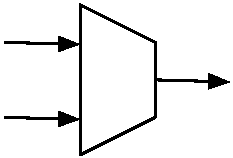
\includegraphics{figures/mux}

  \caption{A basic 2:1 multiplexor.}
  \label{fig:mux}
\end{figure}


\section{Counting}

Counting is a very basic operation in digital systems. On might count events.
However, more often counting is used to define a time interval. Counting the
clock cycles and triggering an action when the time interval has expired.

A simple approach is counting up to a value. However, in computer science,
and in digital design, counting starts at 0. Therefore, if we want to count till
10 we count from 0 to 9. The following code shows such a counter that counts
till 9 and wraps around to 0 when reaching 9.

If we want to count N, we start with 0 and count till N-1.

\todo{counter code}



This is straight forward. However, one might ask if this is the most efficient
implementation of counting. The comparison agains an end value, 10 in our
example, involves some combinational circuit in an ASIC. More efficient in an
ASIC (and as well in loops of programs) is counting down and exit when 0
is reached.

If we want to count N, we start with N-1 and count till 0.

\todo{down counting code}

With a comparison against 0 we need only a NOR gat to detect the 0 condition.
This optimization is valid for an ASIC, but not for an FPGA based on LUTs.
With comparison using LUTs there is no difference comparing against a '0' or
'1' bit. In that case use the better readable counting logic towards the end value.

However, there is still one more trick a clever hardware designer can pull off.
Counting up or down needed a comparison agains all counting bis, so far.
What about counting down \emph{one to many}? In that case the counter
becomes negative. Detecting a negative value is simply comparing the
most significant bit against 'a'.

If we want to count N, we start with N-2 and count till -1.

\todo{Show optimized down counting code.}


\todo{discuss >= and so on}

\chapter{Build Process and Testing}

Chisel is written in Scala, so any build process that supports Scala is possible
with a Chisel project. One popular build tool for Scala is \href{https://www.scala-sbt.org/}{sbt},
which stands for Scala interactive build tool.
Besides driving the build and test process, \code{sbt} also downloads the correct
version of Scala and the Chisel libraries.

The Scala library that represents Chisel and the Chisel testers are automatically
downloaded during the build process from a Maven repository.
The libraries are referenced by \code{build.sbt}. It is possible to configure \code{build.sbt}
with \code{latest.release} to always use the most actual version of Chisel.
However, this means on each build the version is looked up from the Maven
repository and an Internet connection is needed for the build to succeed.
Better use a dedicated version of Chisel and all other Scala libraries in your \code{build.sbt}.
Maybe sometimes it is also good to be able to write hardware code and test it without Internet connection.
For example, it is cool to do hardware design on a plane.

\chapter{Components}

A larger digital design is structured into a set of components, structured in
a hierarchical way. Each component has an interface with input and output
wires. These are similar to input and output pins in an IC.
Components are connected by by wiring up the inputs and outputs.
Components are may contain subcomponents to build the hierarchy.

Hardware components are called modules in Chisel. Each module extends
the class \code{Module} and contains a field \code{io} for the interface.
The interface is defined by a \code{Bundle} that is wrapped into a call to \code{IO()}.
The \code{Bundle} contains fields to represent input and output pins of
module. The direction is given by wrapping a field into either a call to \code{Input()}
or \code{Output()}. The direction is from the view of the component itself.

In this section we explore some medium sizes digital designs, such as
a FIFO buffer, which are used as building blocks for larger design.
As an example we will design a serial interface (also called UART),
which itself will use the FIFO buffer.

\section{FIFO Buffer}

To decouple a write (sender) and a reader (receiver) some form
of buffering between the writer and the reader is inserted.
A common buffer is a first-in, first-out
(\href{https://en.wikipedia.org/wiki/FIFO_%28computing_and_electronics%29}{FIFO})
buffer. Figure~\ref{fig:fifo} shows a writer, the FIFO, and a reader.
Data is put into the FIFO by the writer on \code{din} with an active
\code{write} signal. Data is read from the the FIFO by the reader on
\code{dout} with an active \code{read} signal.

\begin{figure}
  \centering
  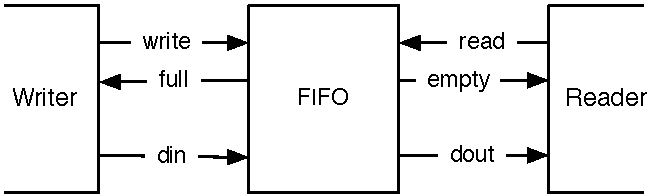
\includegraphics{figures/fifo}

  \caption{A writer, a FIFO buffer, and a reader.}
  \label{fig:fifo}
\end{figure}

A FIFO is initially empty, singled by the \code{empty} signal. Reading
from an empty FIFO is usually undefined. When data is written and never
read a FIFO will become \code{full}. Writing to a full FIFO is usually ignored
and the data lost. In other words, the signals \code{empty} and \code{full}
serve as handshake signals 

Several different implementations of a FIFO are possible: E.g., using on-chip
memory and read and write pointers or simply a chain of registers with a
tiny state machine. For small buffers (up to tens of elements) a FIFO organized
with individual registers connected into a chain of buffers is a simple and efficient
implementation.

We start by defining the IO signals for the writer and the reader. The size of
the data is configurable with \code{size}.

\begin{chisel}
class WriterIO(size: Int) extends Bundle {
  val din = UInt(INPUT, size)
  val write = Bool(INPUT)
  val full = Bool(OUTPUT)
}

class ReaderIO(size: Int) extends Bundle {
  val dout = UInt(OUTPUT, size)
  val read = Bool(INPUT)
  val empty = Bool(OUTPUT)
}
\end{chisel}

\chapter{Chisel 2}

This book covers version 3 of Chisel. And Chisel 3 is recommended for new designs.
However, there is still Chisel 2 code out in the wild, which has not yet been converted
to Chisel 3. There is documentation available how to convert a Chisel 2 project to
Chisel 3:

\begin{itemize}
\item \href{https://github.com/freechipsproject/chisel3/wiki/Chisel3-vs-Chisel2}{Chisel2 vs. Chisel3} and
\item \href{https://github.com/schoeberl/chisel-examples/blob/master/TowardsChisel3.md}{Towards Chisel 3}
\end{itemize}

However, you might get involved in a project that still uses Chisel 2,
e.g., the \url{https://github.com/t-crest/patmos}{Patmos} processor.
Therefore, we will provide here some information on Chisel 2 coding for those who
have started with Chisel 3.

First, all documentation on Chisel 2 has been removed from the web sites
belonging to Chisel. We have rescued those PDF documents and put them
on GitHub at \url{https://github.com/schoeberl/chisel2-doc}.
You can use the Chisel 2 tutorial by switching to the Chisel 2 branch:

\begin{chisel}
git clone https://github.com/ucb-bar/chisel-tutorial.git
cd chisel-tutorial
git checkout chisel2
\end{chisel}

The main visible difference between Chisel 3 and 2 are: the definitions of
constants, bundles for IO, wires, memories, and probably older forms of register
definitions.

Chisel 2 constructs can be used, to some extend, in a Chisel 3 project by
using the compatibility layer using as package \code{Chisel} instead of \code{chisel3}.
However, using this compatibility layer should only be used in a transition phase.
Therefore, we will not cover it here.

Here are two examples of basic components, the same that have been presented
for Chisel 3. A module containing combinational logic:

\lstinputlisting[language=chisel]{chisel2/src/main/scala/Logic.scala}

Note that the \code{Bundle} for the the IO definition is \emph{not} wrapped into
an \code{IO()} class.  Furthermore, the direction of the different IO ports is defined
as part of type definition, in this example as \code{INPUT} and \code{OUTPUT}
as part of \code{UInt}. The width is given as the second parameter.

\begin{minipage}{\linewidth}
The 8-bit register example in Chisel 2:

\lstinputlisting[language=chisel]{chisel2/src/main/scala/Register.scala}
\end{minipage}

Here you see a typical register definition with a reset value passed in as
an \code{UInt} to the named parameter \code{init}. This form is still valid in Chisel 3,
but usage of \code{RegInit} and \code{RegNext} is recommended for new Chisel 3 designs.
Note also here the constant definition of an 8-bit wide 0 as \code{UInt(0, 8)}.

Chisel based testing and Verilog code is generated by calling \code{chiselMainTest}
and \code{chiselMain}. Both ``main'' functions take String array for further parameters.

\lstinputlisting[language=chisel]{chisel2/src/main/scala/LogicTester.scala}

\lstinputlisting[language=chisel]{chisel2/src/main/scala/LogicHardware.scala}

A memory with sequential registered read and write ports is defined in Chisel 2 as:

\begin{chisel}
  val mem = Mem(UInt(width = 8), 256, seqRead = true)
  val rdData = mem(Reg(next = rdAddr))
  when(wrEna) {
    mem(wrAddr) := wrData
  }
\end{chisel}



\section{SBT and Eclipse}

Use an IDE, such as Eclipse, but generate the project with \code{sbt}
from the library dependency description. E.g.,:

\todo{add Eclipse stuff here.}

``sbt eclipse'' and project import

\chapter{Conclusion}
\label{sec:conclusion}

\subsection*{Acknowledgment}

\todo{Sometimes we received some help. Sometimes external funding.}



\section*{Source Access}

All code examples are available in open source from:

\url{https://github.com/schoeberl/chisel-examples}

This book and slides are available in open source from:

\url{https://github.com/schoeberl/chisel-book}

\bibliographystyle{plain}
% Please do not add any references to msbib.bib.
% They get lost when I 'generate' is again (see Makefile)
\bibliography{chisel}

\chapter*{Snippets and Collect Stuff to Describe}

Concatenation and subfield access. Cat is in util. 

\todo{A collection is Chisel snippets collected along some coding}

Initialize a \code{Vec} from a Scala array:
\begin{chisel}
  val program = new Array[Bits](3)
  program(0) = Bits(0x01, 8)
  program(1) = Bits(0x23, 8)
  program(2) = Bits(0x16, 8)
    
  val rom = Vec(program)
\end{chisel}

State machine:
\begin{chisel}
  val fetch :: execute :: load :: Nil = Enum(UInt(), 3)
  val stateReg = Reg(init = fetch)

  switch(stateReg) {
    is(fetch) {
      stateReg := execute
    }
    is(execute) {
      when(isLoad) {
        stateReg := load
      }.otherwise {
        stateReg := fetch
      }
    }
    is(load) {
      stateReg := fetch
    }
  }
\end{chisel}

\textbf{No default assignment possible when declaring a signal! Need an extra one.}




\end{document}

\subsection*{Course Abstract}

Chisel is a hardware construction language implemented as a domain specific language in Scala. Therefore, the full power of a modern programming language is available to describe hardware and, more important, hardware generators. Chisel has been developed at UC Berkeley and successfully used for several tape outs of RISC-V. Here at DTU we used Chisel in the T-CREST project and in teaching advanced computer architecture.

In this course I will give an overview of Chisel to describe circuits at the RTL, how to use the Chisel tester functionality to test and simulate digital circuits, present how to synthesize circuits for an FPGA, and present advanced functionality of Chisel for the description of circuit generators. Besides lecturing we will have lab sessions to describe small circuits and evaluate them in an FPGA.

The aim of the course is to get a basic understanding of a modern hardware description language and be able to describe simple circuits in Chisel. This course shall give a basis to explore more advanced concepts of circuit generators written in Chisel/Scala.

%\begin{figure}
%  \centering
%  \includegraphics{figures/broken-mux}
%
%  \caption{An inkscape figure. With arrows shooting over the destination coordinates!}
%  \label{fig:mux}
%\end{figure}